\documentclass[a4paper]{article}

\usepackage{tikz}
\usepackage{amsmath}
\usetikzlibrary{bayesnet}
\usepackage{caption, subcaption}

\begin{document}

% node:       \node[type](name){caption}
% factor:     \factor[options]{name}{caption}{in}{out}
% plate:      \plate[options]{name}{fitlist}{caption}
% edge:       \edge[options]{inputs}{outputs}
% factoredge: \factoredge[options]{inputs}{factor}{outputs}

\begin{figure}[ht]
  \begin{center}
  \begin{tabular}{ccc}

    % 1st
    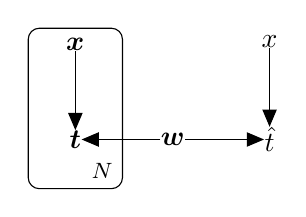
\begin{tikzpicture}

      % Define nodes
	  \node[const]                             (x) {$\quad\boldsymbol{x}\quad$};   % make it wider for enough plate width
	  \node[const, below=of x]                 (t) {$\boldsymbol{t}$};
	  \node[const, right=of t]                 (w) {$\boldsymbol{w}$};
    \node[const, right=of w]                 (t-hat) {$\hat{t}$};
    \node[const, above=of t-hat]             (x-hat) {$x$};

	  % Connect the nodes
	  \edge {x,w} {t} ;
	  \edge {x-hat,w} {t-hat} ;

	  % Plates
	  \plate {xt} {(x)(t)} {$N$} ;

	\end{tikzpicture}
  & \quad

  % 2nd
  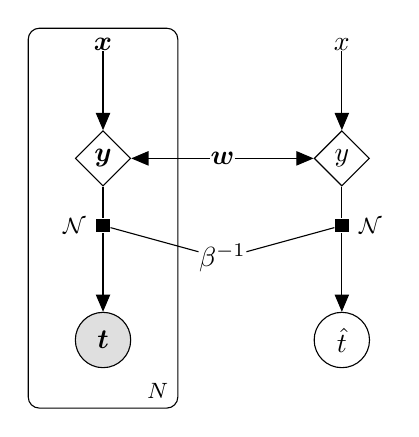
\begin{tikzpicture}

    % Define nodes
    \node[const]                             (x) {$\qquad\boldsymbol{x}\qquad$};
    \node[det, below=of x]                   (y) {$\boldsymbol{y}$};
    \node[const, right=of y]                 (w) {$\boldsymbol{w}$};
    \node[const, below=of w]                 (beta) {$\beta^{-1}$};
    \node[det, right=of w]                   (y-hat) {$y$};
    \node[const, above=of y-hat]             (x-hat) {$x$};
    \factor[below=of y]{t-f}{left:$\mathcal{N}$}{}{};
    \factor[below=of y-hat]{t-hat-f}{right:$\mathcal{N}$}{}{};
    \node[obs, below=of t-f]                 (t) {$\boldsymbol{t}$};
    \node[latent, below=of t-hat-f]          (t-hat) {$\hat{t}$};

    % Connect the nodes
    \edge {x,w} {y} ;
    \edge {x-hat,w} {y-hat} ;
    \factoredge{y,beta}{t-f}{t}
    \factoredge{y-hat,beta}{t-hat-f}{t-hat}

    % Plates
    \plate {xt} {(x)(y)(t-f)(t-f-caption)(t)(y.east)} {$N$} ;

  \end{tikzpicture}

  & \quad

  % 3rd
  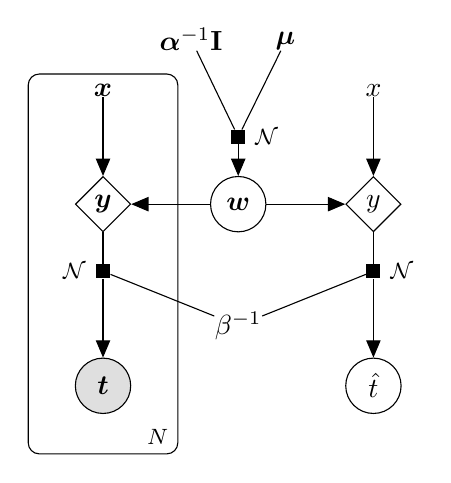
\begin{tikzpicture}

    % Define nodes
    \node[const]                             (x) {$\qquad\boldsymbol{x}\qquad$};
    \node[det, below=of x]                   (y) {$\boldsymbol{y}$};
    \node[latent, right=of y]                (w) {$\boldsymbol{w}$};
    \node[const, below=of w]                 (beta) {$\beta^{-1}$};
    \node[det, right=of w]                   (y-hat) {$y$};
    \node[const, above=of y-hat]             (x-hat) {$x$};
    \factor[above=of w]{w-f}{right:$\mathcal{N}$}{}{};
    \node[const, above=of w-f, xshift=.6cm]  (mu) {$\boldsymbol{\mu}$};
    \node[const, above=of w-f, xshift=-.6cm]   (alpha) {$\boldsymbol{\alpha}^{-1}\mathbf{I}$};
    \factor[below=of y]{t-f}{left:$\mathcal{N}$}{}{};
    \factor[below=of y-hat]{hat-f}{right:$\mathcal{N}$}{}{};
    \node[obs, below=of t-f]                   (t) {$\boldsymbol{t}$};
    \node[latent, below=of hat-f]                 (t-hat) {$\hat{t}$};

    % Connect the nodes
    \edge {x,w} {y} ;
    \edge {x-hat,w} {y-hat} ;
    \factoredge{mu, alpha}{w-f}{w}
    \factoredge{y,beta}{t-f}{t}
    \factoredge{y-hat,beta}{hat-f}{t-hat}

    % Plates
    \plate {xt} {(x)(y)(t-f)(t-f-caption)(t)(y.east)} {$N$} ;

  \end{tikzpicture}
  \\
  \\(a). LSE & (b) MLE & (c) MAP \& Full Bayesian

  \end{tabular}
  \end{center}
  \caption{Polynomial curve fitting models in PRML:
  (a) Least Square Estimation in \$1.1;
  (b) Maximum Likelihood Estimation (point estimation) in \$2.5;
  (c) Maximum-a-Posteriori estimation (point estimation) in \$2.5 and full bayesian approach in \$2.6}
\end{figure}

\begin{figure}[ht]
  \begin{center}
  \begin{tabular}{ccc}

  % 1st: MLE, under glass
  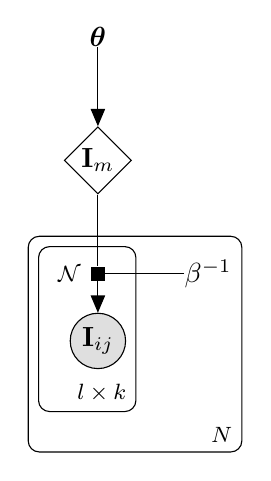
\begin{tikzpicture}

    % Define nodes

    \node[const]                                  (theta){$\boldsymbol{\theta}$}; %
    \node[det, below=of theta]                    (img_model){$\mathbf{I}_m$}; %
    \node[obs, below=1.5 of img_model]            (pix_obs){$\mathbf{I}_{ij}$}; %

    % factors
    \factor[above=of pix_obs]                     {f_obs}{left:$\mathcal{N}$}{}{}; %
    \node[const, right=of f_obs]  (beta){$\beta^{-1}$}; %
    \factoredge {img_model, beta} {f_obs} {pix_obs}; %

    % Connect the nodes
    \edge {theta} {img_model} ;

    % Plates
    \plate {plate_pix_obs} {(pix_obs)(f_obs)(f_obs-caption)} {$l\times k$} ;
    \plate {plate_img_obs} {(plate_pix_obs)(beta)} {$N$} ;

  \end{tikzpicture}

  & \quad

  % 2nd: MAP, under glass
  \begin{tikzpicture}

    % Define nodes

    \node[latent]                                 (theta){$\boldsymbol{\theta}$}; %
    \node[const, above=of theta, xshift=-0.5cm]   (mu){$\boldsymbol{\mu}$}; %
    \node[const, above=of theta, xshift=0.5cm]    (alpha){$\boldsymbol{\alpha}^{-1}\mathbf{I}$}; %
    \node[det, below=of theta]                    (img_model){$\mathbf{I}_m$}; %
    \node[obs, below=1.5 of img_model]            (pix_obs){$\mathbf{I}_{ij}$}; %

    % factors
    \factor[above=of theta]                       {f_theta}{left:$\mathcal{N}$}{}{}; %
    \factor[above=of pix_obs]                     {f_obs}{left:$\mathcal{N}$}{}{}; %
    \node[const, right=of f_obs]  (beta){$\beta^{-1}$}; %
    \factoredge {mu, alpha} {f_theta} {theta}; %
    \factoredge {img_model, beta} {f_obs} {pix_obs}; %

    % Connect the nodes
    \edge {theta} {img_model} ;

    % Plates
    \plate {plate_obs} {(pix_obs)(f_obs)(f_obs-caption)} {$l\times k$} ;
    \plate {plate_img_obs} {(plate_pix_obs)(beta)} {$N$} ;

  \end{tikzpicture}

  & \quad

  % 3rd: FOD, including biased noise due to reflection effects
  \begin{tikzpicture}

    % Define nodes

    \node[latent]                                 (theta){$\boldsymbol{\theta}$}; %
    \node[const, right=of theta]                  (phi){$\boldsymbol{\varphi}$}; %
    \node[const, above=of theta, xshift=-0.5cm]   (mu){$\boldsymbol{\mu}$}; %
    \node[const, above=of theta, xshift=0.5cm]    (alpha){$\boldsymbol{\alpha}^{-1}\mathbf{I}$}; %
    \node[det, below=of theta]                    (img_model){$\mathbf{I}_m$}; %
    \node[obs, below=1.5 of img_model]            (pix_obs){$\mathbf{I}_{ij}$}; %

    % factors
    \factor[above=of theta]                       {f_theta}{left:$\mathcal{N}$}{}{}; %
    \factor[above=of pix_obs]                     {f_obs}{left:$\mathcal{N}$}{}{}; %
    \node[const, right=of f_obs]  (beta){$\beta^{-1}$}; %
    \factoredge {mu, alpha} {f_theta} {theta}; %
    \factoredge {img_model, beta} {f_obs} {pix_obs}; %

    % Connect the nodes
    \edge {theta,phi} {img_model} ;

    % Plates
    \plate {plate_obs} {(pix_obs)(f_obs)(f_obs-caption)} {$l\times k$} ;
    \plate {plate_img_obs} {(plate_pix_obs)(beta)} {$N$} ;

  \end{tikzpicture}


  \\
  \\(a) Under Glass (MLE) &
    (b) Under Glass (MAP) &
    (c) FOD

  \end{tabular}
  \end{center}
  \caption{MAPIS models: $\boldsymbol{\theta}=\{\mathrm{pitch, angle, tlx, tly}\}$, $\alpha^{-1}\mathbf{I}$ is the covariance matrix for $\boldsymbol{\theta}$;
  $\mathbf{I}_m$ is the 8-bit grey image generated by the model (the image dimension is $l\times k$); $\mathbf{I}_{ij}$ are observed pixel intensity at $(i,j)$ in the image captured by sensor;
  $\beta^{-1}$ is the variance of Gaussian noise added to each pixel of $\mathbf{I}_m$ (due to sensor noise and other effects). (a) MLE point estimation for $\boldsymbol{\theta}$;
  (b) MAP point estimation for $\boldsymbol{\theta}$; (c) Adding $\boldsymbol{\varphi}=\{?\}$ as the cause for biased noise due to reflections...}
\end{figure}


\end{document}
